\documentclass[11pt]{scrartcl}
\usepackage[utf8]{inputenc}
\usepackage{mathtools}
\usepackage{amssymb}
\usepackage{listings}
\usepackage{bm}
\usepackage{graphicx}
\usepackage{qtree}
\lstset
{ %Formatting for code in appendix
	language=Matlab,
	basicstyle=\footnotesize,
	numbers=left,
	stepnumber=1,
	showstringspaces=false,
	tabsize=1,
	breaklines=true,
	breakatwhitespace=false,
}
\begin{document}
\centerline{\LARGE{\textbf{CSE881 HW3}}}
\centerline{\large{\textit{Nan Cao,\  A52871775}}}
\centerline{\large{\textit{Oct 4th, 2016}}}
% \maketitle
\section*{Problem 1}
\textbf{(a)}\\
(i)\\
Please see the codes in the last part of this pdf.\\
(ii)\\
Please see the codes in the last part of this pdf.\\
(iii)\\
Use the codes in "Q1.m", we can mathematically find the following combination of non-linearly independent column pairs.\\
( 4, 35); ( 4, 36); ( 4, 37); ( 22, 35); ( 22, 36); ( 22, 37); ( 30, 35); ( 30, 36); ( 30, 37); ( 31, 35); ( 31, 36); ( 31, 37); ( 32, 35); ( 32, 36); ( 32, 37); ( 33, 35); ( 33, 36); ( 33, 37); ( 34, 35); ( 34, 36); ( 34, 37); ( 35, 37); ( 35, 38); ( 35, 39); ( 35, 40); ( 35, 41); ( 35, 42); ( 35, 47); ( 35, 48); ( 36, 37); ( 36, 38); ( 36, 39); ( 36, 40); ( 36, 41); ( 36, 42); ( 36, 47); ( 36, 48); ( 37, 38); ( 37, 39); ( 37, 40); ( 37, 41); ( 37, 42); ( 37, 47); ( 37, 48).\\
Only group 4 that contains both of the columns in a pair.\\
Following are the names of columns:\\
    30. weekday  is  monday:             Was the article published on a Monday?\\
    31. weekday  is  tuesday:            Was the article published on a Tuesday?\\
    32. weekday  is  wednesday:          Was the article published on a Wednesday?\\
    33. weekday  is  thursday:           Was the article published on a Thursday?\\
    34. weekday  is  friday:             Was the article published on a Friday?\\
    35. weekday  is  saturday:           Was the article published on a Saturday?\\
    36. weekday  is  sunday:             Was the article published on a Sunday?\\
    37. is  weekend:                    Was the article published on the weekend?\\
Mathematically, all of following are correct answers:\\
( 30, 35); ( 30, 36); ( 30, 37); ( 31, 35); ( 31, 36); ( 31, 37); ( 32, 35); ( 32, 36); ( 32, 37); ( 33, 35); ( 33, 36); ( 33, 37); ( 34, 35); ( 34, 36); ( 34, 37); ( 35, 37); ( 36, 37)\\
\\
And I picked (36,37) as my answer. Firstly, it's mathematically correct. Secondly, the remaining variables show us an aesthetic feeling of mathematics.\\
iv)\\
Please see the codes in the last part of this pdf.\\
\\
\textbf{(b)}\\
\begin{figure} 
	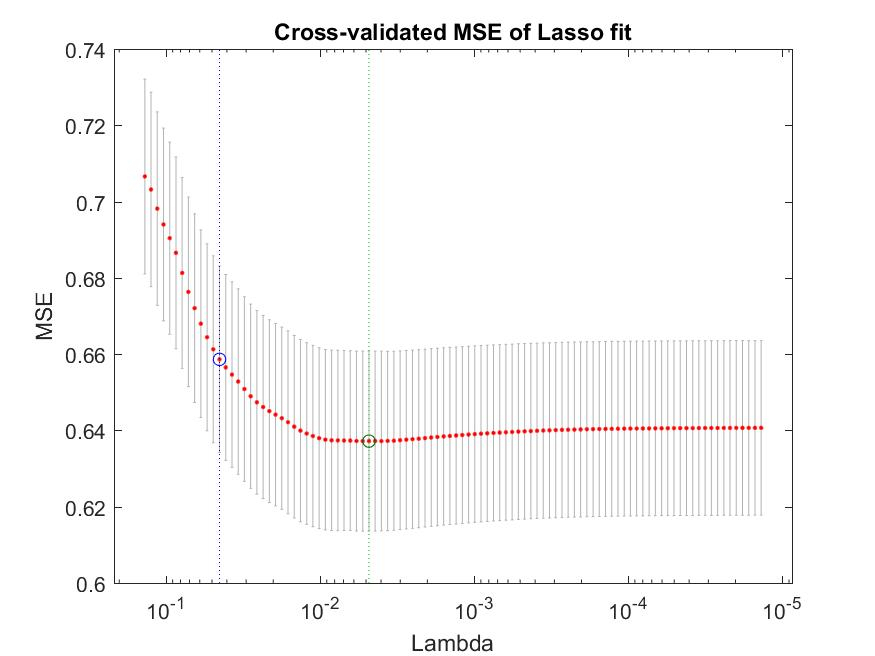
\includegraphics[width=5.5in,height=3.5in]{Q1b.jpg}
	\caption{Problem 2b-lasso}
\end{figure}
The correlation of MLR is -0.0339\\
The correlation of lasso is -0.229\\
The Top 10\\
Top 10 Para of MLR\=1.0e+06
\(4.5335,4.1681,2.6387,0.2139,0.2008,0.1887,0.1764,0.1423,0.000,0.0000\)\\
Col number=\(45,46,4,40,39,36,38,37,57,16\)\\
Top 10 Para of Lass=\(0.0814,0.0736,0.0433,0.0424,0.0327,0.0235,0.0192,0.01,0,0.0159,0.0039\)\\
Col number=\(35,15,27,16,26,56,38,14,13,30\)\\
\textbf{(c)}
THe correlation of kernel is -0.082\\
\textbf{(d)}
all 3 correlations (MLR lasso kernel) remain the same.\\
\section*{Problem 2}
\textbf{(a)}\\
An outlier may have an unusual X or Y. An outlier is an influential point that have great effects on the slope of a regression model. If there are more than 1 outlier, their effect may be quite small, if the effect can be canceled by other's. For example:\\
x1=\(1,2,3,4,5,6\)\ \ \ \ \ \ \ 
y1=\(2.1,3.9,6.1,8.1,10.2,12.3\)\\
x2=\(1,2,3,4,5,6,7\)\ \ \ \ 
y2=\(2.1,3.9,6.1,8.1,10.2,12.3,30\)\\
x3=\(1,2,3,4,5,6,7\)\ \ \ \ 
y3=\(2.1,3.9,6.1,8.1,10.2,12.3,3\)\\
\begin{figure} 
	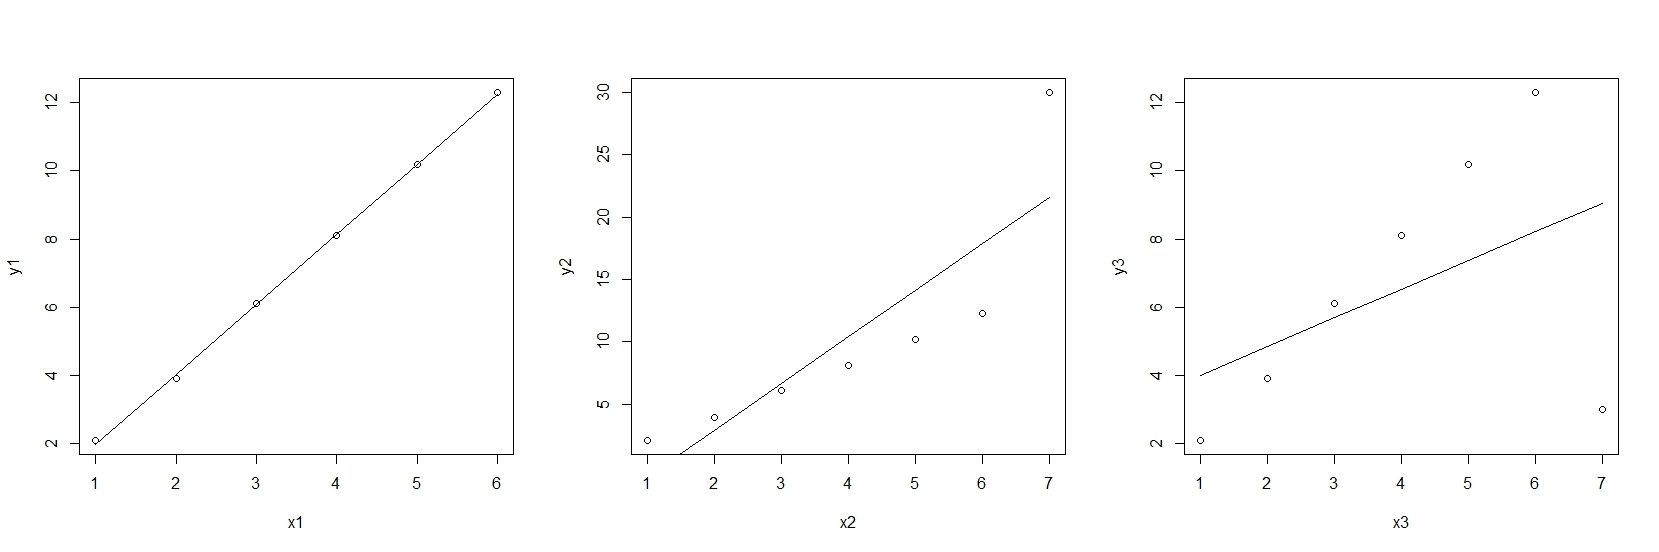
\includegraphics[width=5.5in,height=1.6in]{Q2a.jpg}
	\caption{Problem 3c-2}
\end{figure}\\
\textbf{(b)}\\
\begin{equation*}
\begin{aligned}
&min\sum a_i(y_i-w^T x_i)^2+\lambda||w||\\
&=min(\sqrt{a_i}y_i-w^T \sqrt{a_i}_x_i)+\lambda||w||\\
so\ \ &let\ X^*\ denote\ (\sqrt{a_1} x_1,\sqrt{a_2} x_2,...,\sqrt{a_n} x_n)\\
&let\ Y^*\ denote\ (\sqrt{a_1} y_1,\sqrt{a_2} y_2,...,\sqrt{a_n} y_n)\\
w&=[X^{*T} X^* +\lambda I]^{-1} X^{*T}y^*
\end{aligned}
\end{equation*}
\section*{Problem 3}
\begin{equation*}
\begin{aligned}
E(Sample)&=-\frac{1}{2}log_{2}\frac{1}{2}-\frac{1}{2}log_{2}\frac{1}{2}\\
&=1\\
E(A)&=\frac{1}{2}(-\frac{2}{3}log_{2}\frac{2}{3}-\frac{1}{3}log_{2}\frac{1}{3})\\
&=0.9183\\
E(B)&=
\frac{1}{3}(-\frac{1}{2}log_{2}\frac{1}{2}-\frac{1}{2}log_{2}\frac{1}{2})
+\frac{1}{12}(-\frac{5}{5}log_{5}\frac{5}{5}-\frac{0}{5}log_{2}\frac{0}{0})
+\frac{7}{12}(-\frac{3}{7}log_{2}\frac{3}{7}-\frac{4}{7}log_{2}\frac{4}{7})\\
&=0.9081\\
\end{aligned}
\end{equation*}
B is better because 1-E(B) is bigger.\\
\section*{Codes}
\begin{lstlisting}
% NAN CAO CSE881 HW4
% set dir in nan's win lap
cd C:\Users\nan66\Dropbox\CSE881\HW4\;
%set dir in nan's linux lap
% cd /home/nan/Dropbox/CSE881/HW4;
%%%%%
%(a)
%%%%%
ONP=csvread('OnlineNewsPopularity.csv',1,0);
Pre=ONP(:,1:58);%col 1~58 as Predict Variable
Tar=ONP(:,59);%col 59 as the Response/Target Variable
Tar=log(Tar);
Tar=Tar(:);
Tar(Tar==-Inf)=0;
rPre=rank(Pre);%rank of Predict Matrix
a=0;%set 3 initial variables
b=0;
c=0;
for i=1:57
for j=(i+1):58 % try all the possible combination of 2 columns
A=Pre;
A(:,j)=[];%remove the one with greater column number first
A(:,i)=[];
rA=rank(A);
if rA==56;
a=a+1;%use a to calculate the number of the possible ij
b(a)=i;%save possible i
c(a)=j;%save possible j
end
end
end
d=[b;c]';%show all the possible combination of removing
d
%Remove column 36(is it Su) and column 37(is it Weekend);
Pre1=Pre;
Rm=[36,37];
Pre1=Pre;
Pre1(:,Rm)=[];
rank(Pre1)
%%%%%
%(b)
%%%%%
Len=length(Tar);
TrainPre=Pre1(1:2000,:);
TrainTar=Tar(1:2000);
TestPre=Pre1(2001:Len,:);
TestTar=Tar(2001:Len);
sTrainPre=zscore(TrainPre);%standardize
sTestPre=zscore(TestPre);
% TrainTar=zscore(TrainTar);%standardize
% TestTar=zscore(TestTar);
TrainPre1 = [TrainPre ones(2000,1)]; % add a column of 1s
sTrainPre1 = [sTrainPre ones(2000,1)]; 
TestPre1 = [TestPre ones(Len-2000,1)]; 
sTestPre1 = [sTestPre ones(Len-2000,1)]; 
%MLR
wMLR=regress(TrainTar,sTrainPre1);
%lasso
[w,stats]=lasso(sTrainPre1,TrainTar,'Alpha',1,'CV',10);
Figure1=lassoPlot(w,stats,'PlotType','CV');
saveas(Figure1,'Q1b','jpeg');
wbest=w(:,stats.Index1SE');

%cal top 10
[a1,b1]=sort(abs(wMLR),'descend');
a1(1:10)
b1(1:10)
[a2,b2]=sort(abs(wbest),'descend');
a2(1:10)
b2(1:10)
%cal  predicted values
MLRPreVal=sTestPre1*wMLR;
CorMLR=corr(MLRPreVal,TestTar)
LasPreVal=sTestPre1*wbest;
CorLas=corr(LasPreVal,TestTar)
%%%%
%(c)
%%%%
Len=length(Tar);
TrainPre=Pre1(1:2000,:);
TrainTar=Tar(1:2000);
TestPre=Pre1(2001:Len,:);
TestTar=Tar(2001:Len);
lambda=0.001
%calculate alpha for function 'applyKernel'
dist1 = pdist(sTrainPre); % calculate distance between every pair of points
dist1 = squareform(dist1); % convert to square matrix
K = exp(-(1e-7) * dist1.^2); % mu: kernel parameter (specified by user)
alpha = inv(K + lambda*eye(2000)) * TrainTar;
pred = applyKernel(sTrainPre,TestPre, alpha,1e-7);
CorKer=corr(pred,TestTar)





%%%%%%%%%%%%%%%%%%%%%%%%%%%%%%%%%%%%%%%%
%(d)
%%%%
Pre2=Pre1;
Pre2(:,18:29)=log(Pre2(:,18:29));
Pre2(Pre2==-Inf)=0;
Len=length(Tar);
TrainPre=Pre2(1:2000,:);
TrainTar=Tar(1:2000);
TestPre=Pre2(2001:Len,:);
TestTar=Tar(2001:Len);
sTrainPre=zscore(TrainPre);%standardize
sTestPre=zscore(TestPre);
TrainPre1 = [TrainPre ones(2000,1)]; % add a column of 1s
sTrainPre1 = [sTrainPre ones(2000,1)]; 
TestPre1 = [sTestPre ones(Len-2000,1)]; 
sTestPre1 = [sTestPre ones(Len-2000,1)]; 
%%%%%%%%%%%%%%%%%%%%%%%%%%%%%%%%%%%%%%%%
%MLR
wMLR=regress(TrainTar,sTrainPre1);
%lasso
[w,stats]=lasso(sTrainPre1,TrainTar,'Alpha',1,'CV',10);
Figure1=lassoPlot(w,stats,'PlotType','CV');
saveas(Figure1,'Q1d','jpeg');
wbest=w(:,stats.Index1SE');

% %cal top 10
% [a1,b1]=sort(abs(wMLR),'descend');
% a1(1:10)
% b1(1:10)
% [a2,b2]=sort(abs(wbest),'descend');
% a2(1:10)
% b2(1:10)
%cal  predicted values
MLRPreVal=sTestPre1*wMLR;
CorMLR2=corr(MLRPreVal,TestTar)
LasPreVal=sTestPre1*wbest;
CorLas2=corr(LasPreVal,TestTar)
%%%%
%(c)
%%%%
Len=length(Tar);
TrainPre=Pre1(1:2000,:);
TrainTar=Tar(1:2000);
TestPre=Pre1(2001:Len,:);
TestTar=Tar(2001:Len);
lambda=0.1;
%calculate alpha for function 'applyKernel'
dist1 = pdist(sTrainPre); % calculate distance between every pair of points
dist1 = squareform(dist1); % convert to square matrix
K = exp(-(1e-7) * dist1.^2); % mu: kernel parameter (specified by user)
alpha = inv(K + lambda*eye(2000)) * TrainTar;
pred = applyKernel(sTrainPre,TestPre, alpha,1e-7);
CorKer2=corr(pred,TestTar)
\end{lstlisting}
\end{document}